\documentclass[tikz,border=7pt]{standalone}
\usepackage{amsmath}
\usetikzlibrary{arrows.meta,positioning,calc}

\tikzset{
  component/.style={
    draw,
    rectangle,
    minimum width=25mm,
    minimum height=12mm,
    align=center
  },
  controller/.style={
    draw,
    rectangle,
    rounded corners=2pt,
    minimum width=25mm,
    minimum height=12mm,
    align=center
  },
  sum/.style={
    draw,
    circle,
    minimum size=7mm,
    inner sep=0pt
  },
  signal/.style={
    -{Latex[length=2.2mm]},
    thick
  }
}

\begin{document}
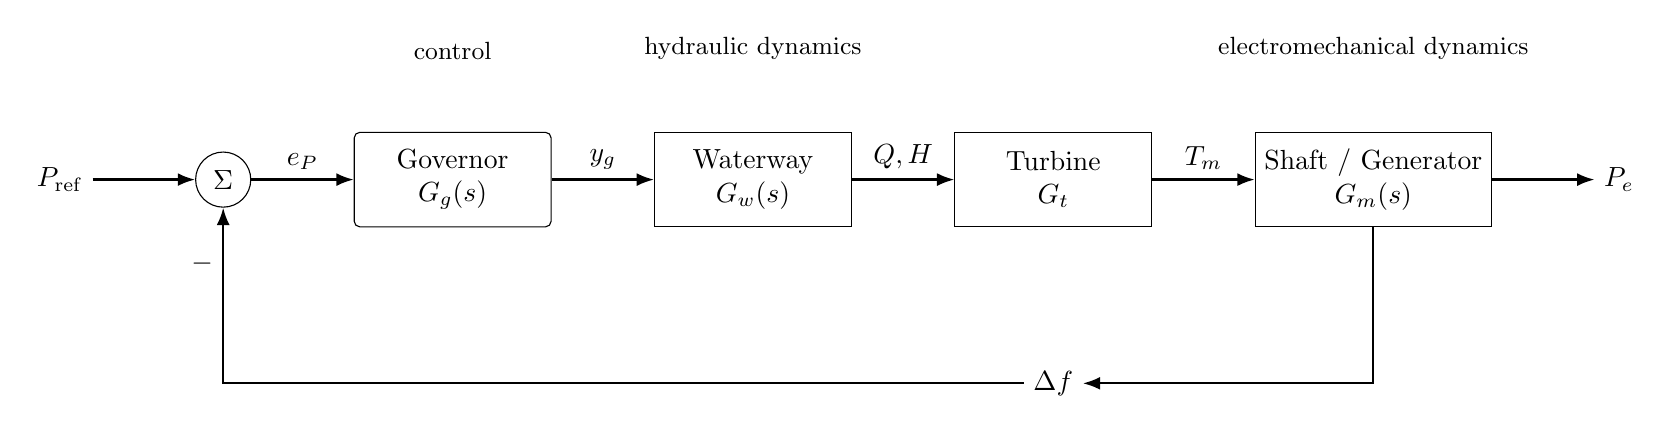
\begin{tikzpicture}[node distance=12mm and 13mm]

\node (pref) {$P_{\mathrm{ref}}$};
\node[sum, right=of pref] (sum) {$\Sigma$};
\node[controller, right=of sum] (gov) {Governor\\$G_g(s)$};
\node[component, right=of gov] (water) {Waterway\\$G_w(s)$};
\node[component, right=of water] (turbine) {Turbine\\$G_t$};
\node[component, right=of turbine] (shaft) {Shaft / Generator\\$G_m(s)$};
\node[right=of shaft] (pout) {$P_e$};

\node[below=17mm of turbine] (freq) {$\Delta f$};

\draw[signal] (pref) -- (sum);
\draw[signal] (sum) -- node[above] {$e_P$} (gov);
\draw[signal] (gov) -- node[above] {$y_g$} (water);
\draw[signal] (water) -- node[above] {$Q,H$} (turbine);
\draw[signal] (turbine) -- node[above] {$T_m$} (shaft);
\draw[signal] (shaft) -- (pout);

\draw[signal] (shaft.south) |- (freq);
\draw[signal] (freq) -| node[pos=0.84,left] {$-$} (sum.south);

\node[above=8mm of water, align=center] {\small hydraulic dynamics};
\node[above=8mm of gov, align=center] {\small control};
\node[above=8mm of shaft, align=center] {\small electromechanical dynamics};

\end{tikzpicture}
\end{document}
